\chapter{Foreground Component Separation}
\label{fg_comp}
One of the ways of removing foregrounds from our data is to have a parametric model for the
foregrounds based on known physics and fit the data to these foreground models to get an
estimate of the parameters and use them to eliminate the foregrounds in the data. This is
the methodology followed by Commander pipeline of the Planck collaboration \cite{cmbpara} and LIL Method
\cite{lilrishi}. These methods suffer from being model dependent and the parameters are
insufficient to model the foregrounds because various physical processes
contribute to the foreground in a single pixel, making it hard to model these with a single
parametric model. Therefore, it is useful to look at
algorithms which are model independent and just use the data to estimate the foreground
characteristics.\\
Various such \emph{blind} component separation algorithms have been proposed where
only the spectrum of the signal is needed \cite{ilc,gilc} and have been applied in various
variations such as Harmonic space, Needlet frame etc \cite{harmonicilc, needlet}. Since these
blind algorithms require the number of foreground components to be lesser than the
number of spectral channels available, it is necessary to divide the sky with similar foreground
properties into different regions and apply the algorithm separately on those regions to reduce
the number of foreground components. These existing variations try to divide the data into
different clusters with similar foregrounds based on heuristic arguments and
our current understanding of the
properties of the foregrounds. We provide a spectral data based
approach extending upon this data driven foreground clustering approach \cite{datarishi}, which
uses the signature of the foregrounds available in the data.
Since the data is clustered only based on the spectra, different regions of the sky can still be
in the same cluster based on their foreground properties. To the best of our
knowledge, this is the first attempt at using \emph{unsupervised} machine learning for foreground
component separation.  

\section{Generalized ILC}
We want to separate out the cosmological signal of interest from the different frequency maps provided by the Planck
collaboration, by subtracting out the different foreground signals. The Generalized ILC is used to separate out any signal with a known
spectrum.\\
The observed temperature data, in different pixels(positions) and frequency channels can be written as,
\begin{align}
  T(\nu, p) = S(\nu) A(p) + F(\nu, p) + N(\nu, p)
\end{align}
Where,
\begin{itemize}
   \item $S(\nu)$ is the spectrum of the signal we are looking for.
      This is essentially the unit conversion which let's us perform ILC to extract any signal of a known spectrum.
      For eg, In the case of CMB, in $K_{cmb}$ units, it
      is equal to one. ie, The CMB Temperature is independent of the frequency and is only a function of the pixel $p$.
   \item $A(p)$ is the position dependent signal (sky-map) we are looking for.
   \item $F(\nu, p)$ is the sum of all the foreground components in a particular pixel. Since, different foregrounds with different
      spectra contribute in each pixel, this is dependent on both the frequency and the pixel position in the sky.
   \item $N(\nu, p)$ is the noise which is in general dependent on both the frequency channel and the pixel position.
\end{itemize}

Now, Let us say that the signal is a linear combination of the frequency maps.

\begin{align}
  s_{sig}(p) = \sum\limits_{\nu} w(\nu) T(\nu, p)
\end{align}
knowing that $s_{sig}(p) = A(p)$, in the absence of foregrounds and noise, We see that,
\begin{align}
  \label{constraint}
\sum\limits_\nu  w(\nu) S(\nu) = 1
\end{align}
If we knew the true signal $s_{true}(p)$, We could find the weights ($w(\nu)$) assigned to the
different frequencies by minimising a cost function,
\begin{align}
C &= \sum\limits_p \left( s_{true}(p) - s_{sig}(p) \right)^2\\
C &= \sum\limits_p \sum\limits_{\nu} \left(  F(\nu, p) + N(\nu, p) \right)
\end{align}
Since, We don't know the true value of the signal, Let us consider an alternate cost function
\begin{align}
C^\prime &= \sum\limits_p \left(s_{sig}(p) \right)^2\\
C^\prime &= \sum\limits_p (s_{true}(p))^2 + C - \sum\limits_p s_{true}(p) \sum\limits_{\nu} \left(F(\nu, p) + N(\nu, p)\right)
\end{align}
Since the first term is a additive constant, which is irrelevant to the minimization problem. We see that $C = C^\prime$ if,
the third term is zero (ie, The foregrounds and Noise are not correlated with the signal). Though the Noise is in general not
correlated with the signal, We can't say the same about the foregrounds. This leads to a bias, where the ILC also will remove the
part of the signal correlated with the foregrounds. This results in a solution which has lesser power than the actual signal. \cite{datarishi}

It has also been previously studied that, this ILC Bias is significant only for $l =2$, and is negligible for all the higher multipoles.
It can however, start affecting the higher multipoles if we increase the number of partitions to a high number. \cite{datarishi}

By minimising the cost, with respect to the constraint \eqref{constraint}, We get the following equations for the weight.

\begin{align}
  \begin{split}
    w(i) = \frac{\strut \sum\limits_j D_{ij}^{-1}}{\strut \sum\limits_{ij} D_{ij}^{-1}}
  \end{split}
\end{align}
where,
\begin{align}
  \begin{split}
    D_{ij} \equiv \sum\limits_p T(i, p)T(j, p) 
  \end{split}
\end{align}
and where the sum over the pixels is done for pixels in a single cluster.

\subsection{Combining information from maps with different resolutions}
Different resolution maps, has different information. In order to effectively use
out algorithm, We need to find a way to combine these information effectively. \cite{datarishi}
Since the noise properties depend on the resolution of the map used, We need to rebeam
all the maps to a common resolution. 
But, It is not straightforward to see which resolution map is useful for performing the ILC.
Rebeaming all the maps to a lower resolution means, We loose all the large $\ell$ signals. Whereas,
rebeaming all the maps to a higher resolution means, the noise in the lower resolution gets boosted
significantly, and these noise dominated maps will contribute less to the final solution, 
effectively loosing any information contained in these maps.

We would effectively like a technique, where all the channels with sufficient signal to noise ratio, provide information.
We first rebeam all the maps to gaussian beams with different resolutions. We then adopt the following technique.
\begin{itemize}
\item Rebeam all maps to lowest resolution map and apply FC-ILC
  algorithm. This solution will have the lowest foregrounds at that resolution
  since it uses the information from the maximum number of channels. Let's
  label the ILC solutions by index $a$, i.e. $s^a(p)$, with $a=1$ corresponding to the
  lowest resolution, and $a>b$ implying resolution of map $a$ is higher
  than map $b$. We will denote the corresponding (Gaussian) beams with $b_{\ell}^a$.
\item We, leave the low resolution channels and perform ILC after rebeaming to the next higher resolution.
\item Repeat the above step until not enough frequency channels remain to get a
  viable ILC solution
\item combine the solution in harmonic space, to get
  the final solution $s^f(p)$, or in harmonic space $a_{\ell m}^f$, with the resolution corresponding to the
  highest resolution channel with beam $b_{\ell}^n$, as follows:
\begin{align}
a_{\ell m}^f= 
b_{\ell}^n\left[a_{\ell m}^1+(1-b_{\ell}^{1})\left( a_{\ell m}^{2} + (1-b_{\ell}^{2})
\left(  a_{\ell m}^{3} + ... + \left(1-b_{\ell}^{n-1}\right)\frac{a_{\ell m}^n }{b_{\ell}^n}\right)\right)\right].
\end{align}
In the last term in nested brackets in the above equation, we correct the
highest resolution solution with its beam and then use the resulting
$a_{\ell m}$ to fill in only the information not present in the next lower
resolution map, hence the factor of $(1-b_{\ell}^{n-1})$.
We keep repeating this process to fill-in the information missing from the previous iterations.
\end{itemize}


%\comment{Also write an appendix about the derivation of the formulas} %commented
\section{Quick Introduction to Machine Learning}
Machine learning is a type of an algorithm which, rather than explicitly coding an algorithm for a
particular function/behaviour, gives the computer the ability to \emph{learn} that function. Machine learning involves a
training set, from which the computer \emph{learns} the function of interest, and a validation set where the computer applies
whatever it has learned from the training set and gives us results.
Whenever, We say that the computer \emph{learns}, we mean a minimization of some cost function, by varying the parameters of the
function the computer is trying to learn. This cost function captures the deviation from the desired behavior of the
algorithm after learning. 

We would be particularly interested in a classifier,
which can be defined as a function ($f: \mathcal{D} \rightarrow [0,1]^n$) which divides the input data (from the domain $\mathcal{D}$
which is usually $\mathbb{R}^m$) into $n$ different classes, by assigning
a probability for each of the classes. 

We would also be only implementing hard clustering, where the final result is a single cluster value instead of a set of probabilities for each
cluster. This is implemented by assigning the value of the cluster to be the one with maximum probability. 

In our use case, We will be dividing the sky into different classes based on their foreground properties, while using the different frequencies
as input.

Based on our training set, machine learning can be divided into two categories.
\begin{itemize}
    \item Supervised Machine Learning
    \item Unsupervised Machine Learning
\end{itemize}

\subsection{Supervised Machine Learning}
A machine learning algorithm is said to perform supervised learning, when the training set is different from the validation set, and we
have the expected learning outcomes as part of our training set. These labeled training sets consist of a input and an expected output
value as part of the examples, and the algorithm learns the function which relates the input value to the output value based on these training examples.
In this case, the cost function is some sort of deviation from the output value compared to the given output value in the
training examples.

There have been attempts \cite{fgremovalsupervised} to classify 
the foregrounds in the
data using this approach by using simulations to generate the training set. This method involves using the simulations to
generate the training data for different classes based on the different foreground models used in the simulation. We then expect the machine
learning algorithm to \emph{learn} from these simulations and help us classify the real sky into regions based on it's foreground properties.

This method suffers from being model dependent, similar to the parametric models of component separation
as the algorithm tends to learn only based on the foreground models fed during the
simulation. In order to avoid this, We use unsupervised machine learning which gives us the advantage of clustering the data in a model
independent manner.


\subsection{Unsupervised Machine Learning}
Unsupervised learning is when a machine learning algorithm has no prior information about the data set in terms of a training set and
the data learns and validates from the same set. In this method only the raw data is given to the algorithm, and it tries to \emph{learn}
patterns inherent in the data, without any labels to learn from.

This would be really useful for our purposes since it allows us to partition the sky based on the frequency without any model
dependent inputs.
\\
We would specifically be using clustering algorithms and dimensionality reduction algorithms.
\paragraph{Clustering Algorithms} Partition the data into different classes based on how every data point
is located with respect to it's neighbours. These algorithms have a varying point in the
\emph{data space}\footnote{The space of all possible data} which is representative of the cluster and
assign the cluster to the available data based on it's relationship to this point. 

\paragraph{Dimensionality Reduction}
Clustering algorithms in higher dimensions tend to be heavily dependent on the initial seed for the
clusters. It is therefore, incredibly useful to reduce the dimentionality of the data by summarizing the
information in fewer number of variables and then performing the clustering in a lower dimensional space.

\subsection{Neural Networks}
A neural network is a special case of a machine learning algorithm, which has a specific functional form.
The advantage a neural network provides is based on a mathematical theorem that this specific functional form can
approximate any continuous function \cite{univapproxtheorem}.\\
A single layer neural network is defined by the following function.
\begin{align}
    \vec{c} = \sigma(M_1 \vec{v} + \vec{b_1})
\end{align}
Where, 
\begin{itemize}
\item $\vec{v}$is the Input Data with the dimensionality of our Input variables space
\item $\vec{c}$ is the Output data with the dimensionality of our number of classes
\item $\vec{b}$ is the bias vector with the dimensionality of our number of classes,
\item $\sigma$ is a sigmoidal\footnote{  A sigmoid function is a bounded, differentiable,
    real function that is defined for all real input values and has a non-negative derivative
    at each point. } function which acts component wise. Also known as the activation function
\item $M$ is a matrix whose elements we will tune as parameters
\end{itemize}
We can now, tune the parameters (the elements of the matrix M ) based on a cost function, which after training will
help us get the final matrix, which we can use to classify our data. A multi-layer neural network can be constructed by
composition of this, an arbitary number of times. We use ReLU ($\max(0, x)$) as our activation function. 


\section{New tSZ maps with unsupervised Machine Learning}
\label{tSZmaps}
In unsupervised machine learning, we take the hard clustering approach,
where each data belongs only to a single class. In order to smooth the boundaries of the partitions
like the current ILC algorithms, we repeat the hard clustering multiple times with different seeds.
Since various seeds produce different partitions, and there is no a-priori reason to consider one
partition over the other, we consider all of them with equal probability. We see that this approach
essentially smoothens the boundary and no additional smoothing across the cluster boundaries are
necessary. 

\subsection{`k-means clustering' method}
k-means clustering partitions $n$ data points into $k$ clusters, by associating each point to the
nearest centroid, which serves as a representation of that cluster. By minimising the inertia,
We partition the space into k-regions, which serve as the partition for our clusters to be used in
ILC.
\begin{wrapfigure}{l}{0.5\linewidth}
  \begin{center}
  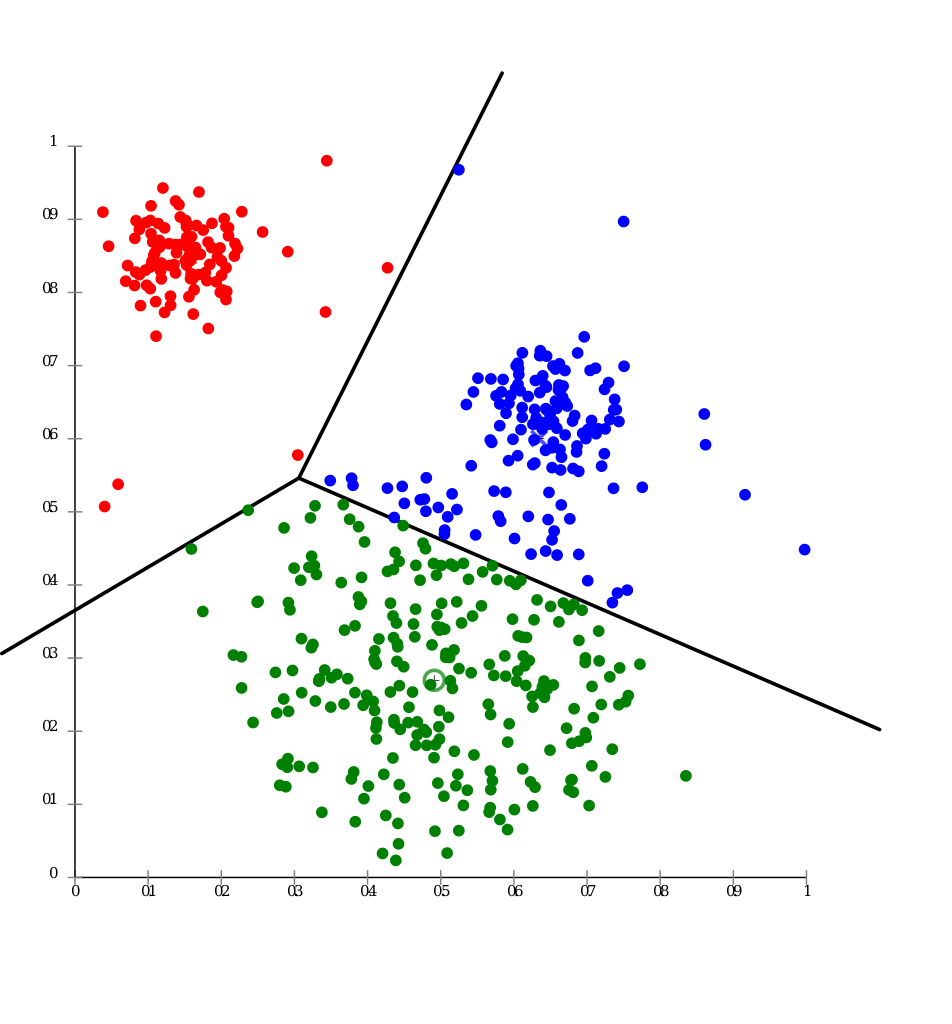
\includegraphics[width = 0.5\linewidth]{kmeans_example.png}
  \end{center}
  \caption{K-Means Clustering Example}
\end{wrapfigure}

The initial positions are initialized using \texttt{k-means++} algorithm in order to avoid the
local minimas, which the random initializations can get into. And the data is rescaled with
quartile scaling, to prevent the outliers from influencing the scaling.
k-means clustering was implemented
using \texttt{scikit-learn} \cite{scikit-learn}

\subsubsection{Choice of Variables for k-means clustering}
Let the frequency maps in $K_{CMB}$ units be denoted by, $T_i$,
where \\$i \in \{30, 44, 70, 100,143, 217, 353, 545, 857\}$Hz.
In order to model the foregrounds, We first subtract the CMB.
$A_i = T_i - T_{100Hz}$. Then we subtract out the tSZ, by changing to the
corresponding $y$ units. The maps we get are mostly dominated by foregrounds.
Apart from clustering these foreground maps separately
(labeled as \emph{raw k-means}),
we divide out the amplitudes of these \emph{raw maps} to make different measures,
which capture how fast the foreground is increasing or decreasing
with frequency similar to the measure defined in the FC-ILC (labelled as \emph{kmeans with m})
\cite{datarishi}.
\\
%\comment{EXPLAIN THESE NUMBERS - WRITE APPENDIX ON UNIT CONVERSION}
  \begin{align}
    \begin{split}
        y_1 = A_{857} - 24.371 A_{143}\quad y_2 = A_{857} - 7.199 A_{217}\quad y_3 = A_{545} - 14.836 A_{143}\\
        y_4 = A_{545} - 4.3826 A_{217}\quad y_5 = A_{353} - 8.215 A_{143}\quad y_6 = A_{353} - 2.4267 A_{217}\\
        y_7 = A_{30} - 1.7339 A_{70}\quad y_8 = A_{44} - 1.541 A_{70}\quad y_9 = A_{217} + 3.671 A_{44}\\
        y_{10} = A_{217} + 5.657 A_{70}\quad y_{11} = A_{353} + 13.73 A_{70}\quad y_{12} = A_{30} - 1.125 A_{44}\\
    \end{split}
  \end{align}
  Apart from clustering these y-maps separately. We divide out the amplitudes to make different
  measures, which capture how fast the foreground is increasing or decreasing with frequency.
  \begin{align}
    \begin{split}
        m_1 = y_1/y_3 \quad m_2 = y_2/y_4 \quad m_3 = y_3/y_5\\
        m_4 = y_4/y_6 \quad m_5 = y_7/y_{12} \quad m_6 = y_{12}/y_5\\
        m_7 = y_7/y_5 \quad m_8 = y_7/y_8 \quad m_9 = y_8/y_5
    \end{split}
  \end{align}
By visually inspecting the maps, We choose the 3 measures. $m_1, m_3, m_7$,
and perform k-means clustering (Appendix:\ref{mmapsappendix})
We also masked the galactic center along with the point sources and clustered
the masked regions separately.
\subsection{Preprocessing}
Before we do machine learning, We need to pre-process the data to remove outliers and heavily contaminated regions.
For this, We first mask the sky and seperate the masked and the un-masked regions. We then perform machine learning on these two regions seperately.
Since all our cost functions are metric based, We need to scale all the different frequency maps into the same range. This makes sure that
all the information in the different frequency maps are used to the same extent. 
\\
While there are many ways to perform this scaling, We specifically use quartile scaling, which is robust to the presence of outliers.
Quartile scaling, scales using the percentile values. In our case, We scale the region between 15-percentile and 85-percentile to a range of 0 to 1. 
This makes sure that all the frequency maps are prioritized equally.

\subsubsection{Masks}
In order to mask the regions which will be dominated by foregrounds, We create masks with different skyfractions. The use the Linearized Iterative Least
squares method \cite{lilrishi} to fit the spectra to a  foreground model and mask the region based on the $\chi^2$ value. \cite{rishimask}
\\
Along side this mask, For all the algorithms, We also mask the outliers (Top and Bottom 1-percentile) in the $m_1, m_3, m_7$ maps\footnote{This is done in order
  to mask radio sources and other point sources}.


\begin{figure}[H]
  \centering
  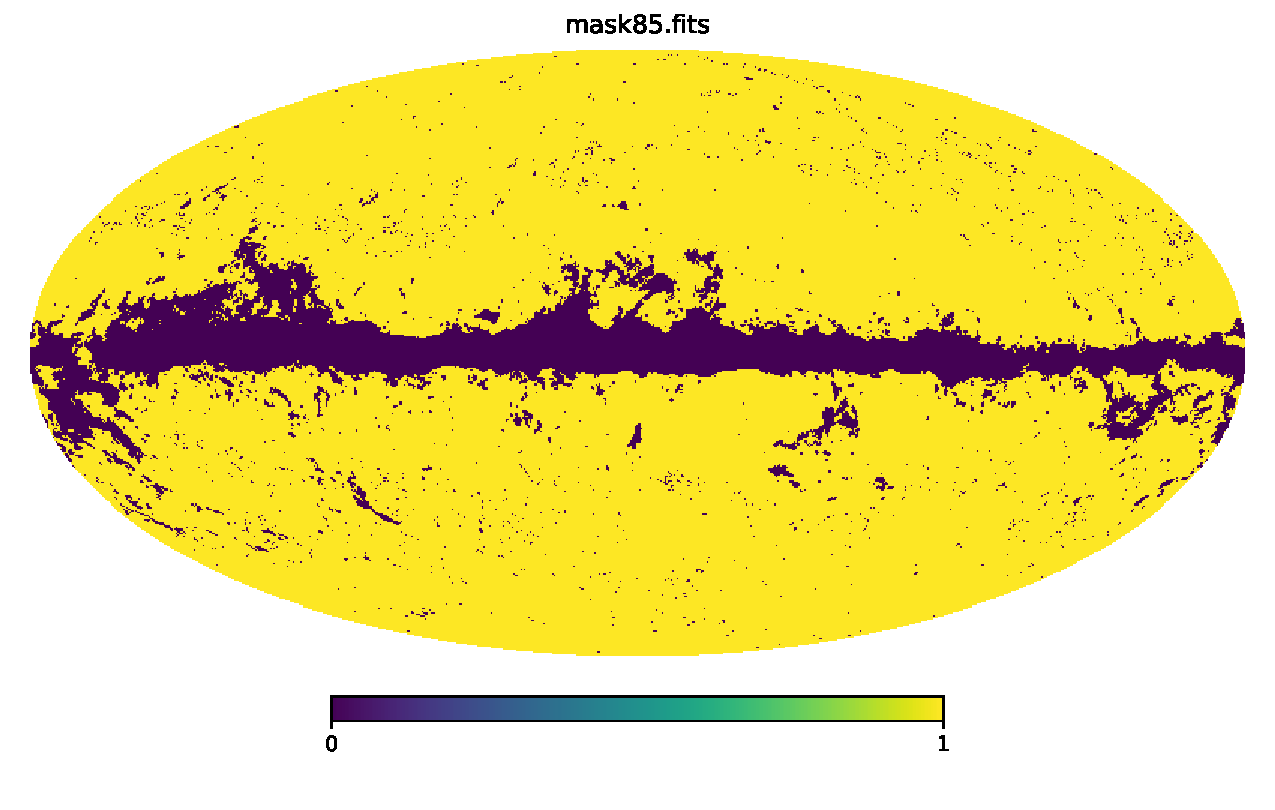
\includegraphics[width = 0.7\linewidth]{mask.pdf}
  \caption{The final Mask}
\end{figure}


While, Calculating the power spectrum, We use a stricter condition on the masks, revealing a lower fraction of the sky. We apodise the masks by replacing the 1s
in the mask by $1 - \exp(-9\theta^2 / (2 \theta_{ap}^2))$ for $\theta < \theta_{ap} = 30'$, the apodization angle, where $\theta$ is the distance from the
nearest masked pixel.

\subsection{Dimensionaliy Reduction}
Since, the choice of parameters is up to us in the previous method, we use non-linear dimensionality
reduction algorithms in order to reduce the 12 dimensional input data (CMB and tSZ
subtracted maps) to a lower dimension in order to
apply the k-means algorithm on it. Unlike the previous method,
we use neural networks to determine the
parameters which encode the maximum information about the data.
We use two non-linear dimensionality
reduction algorithms.\\
The two algorithms used are, 
\begin{itemize}
  \item Auto Encoders
  \item Self Organising Maps
\end{itemize}

\subsection{Auto Encoders}
Auto Encoder is a neural network where, the output dimensionality is the same as input dimentionality.
With a hidden layer having a smaller dimension. We train the network by use the same data for both input and output.
The idea is to make the network learn to reduce the dimentionality to a lower dimension and reconstruct the
input data from that (known as encoder and decoder respectively).
\\
We use a denoising auto encoder, made from an fully connected neural network, using $L^2$-norm as
the cost. There are two intermediate layers for both the encoder and the decoder containing seven and three neurons
each.\\
Once the network has been trained we can use the encoder part for dimensionality reduction.
And then the k-means algorithm is used in this lower dimensional space to cluster the pixels.
Auto encoders were implemented using both \texttt{tensorflow} and \texttt{pytorch} to test out different architectures
\cite{tensorflow, pytorch}.

We vary the learning rate of the neural network by decaying the learning rate, exponentially. The rate of decay is also
considered a hyperparameter. The hyperparameters were tuned by performing a random search trying to minimise the cost as much as
possible.

\subsection{Self Organising Maps}
Self organising map reduces the input data to two dimensions by fitting a discrete two dimensional
manifold on the data and then use k-means algorithm on this manifold.
Self Organising Maps was implemented using the \texttt{somoclu} Library \cite{somoclu}.
We used a 200x200 grid for testing the performance on FFP6 data, and a 300x300 grid for the clustering using the actual Planck Data.

\subsection{Results}
\begin{figure}[H]
  \centering
  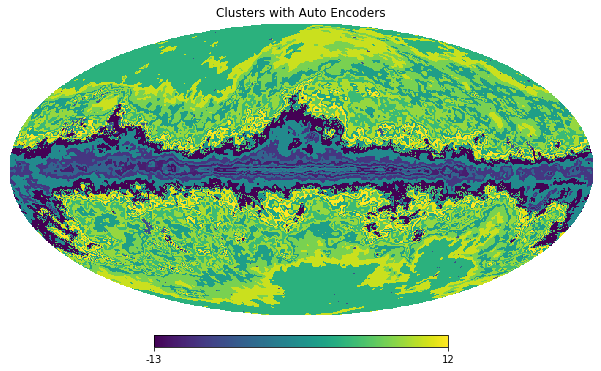
\includegraphics[width=0.35\linewidth]{auto_clusters.png}
  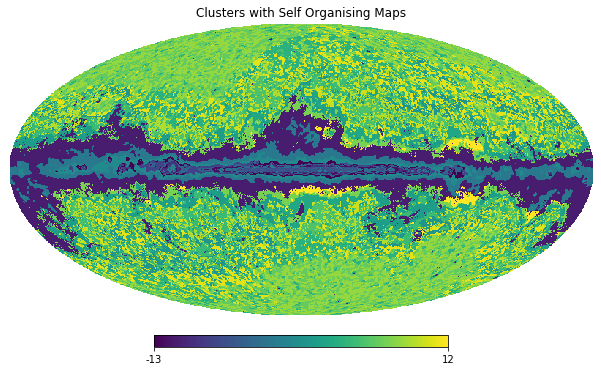
\includegraphics[width=0.35\linewidth]{som_clusters.png}
  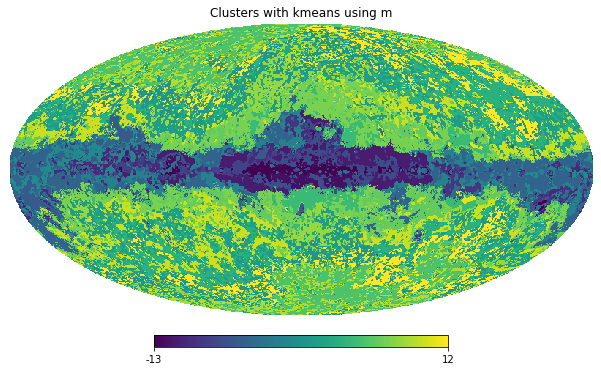
\includegraphics[width=0.35\linewidth]{kmeans_clusters.png}
  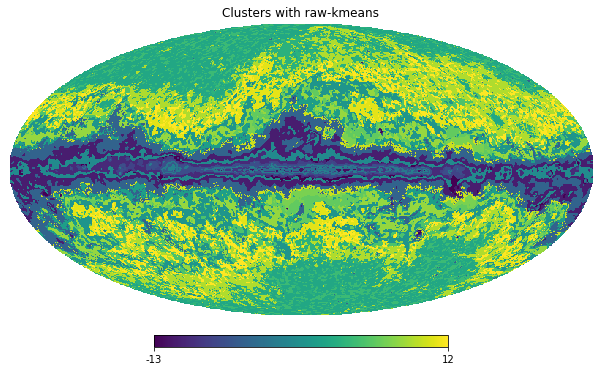
\includegraphics[width=0.35\linewidth]{raw_kmeans_clusters.png}
  \caption{A single instance Clustering of the Sky based on foregrounds using various methods (negative values indicate masked regions)}
\end{figure}
      The result of using the various algoritms FFP6 simulations is shown in Fig(\ref{ffp6res}).
We see that our clustering algorithm is better than the one dimensional version \cite{datarishi}.
We hope to compare it with the existing algorithms using FFP6 simulations. We also see that the
neural network method like self organising map with a 200x200 grid performs, very close to the
k-means algorithm where the measures are chosen by hand. It is interesting to note that
\emph{raw-kmeans} performs the same as a self organising map.
\begin{figure}[H]
  \label{ffp6res}
  \centering
  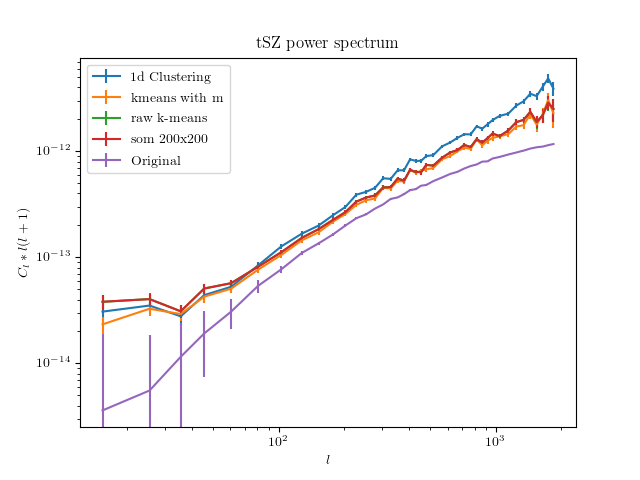
\includegraphics[width=0.7\linewidth]{cl_plots.png}
  \caption{Comparison of the tSZ power spectrum for various methods}
\end{figure}

Seeing that the k-means algorithm using the measures, performs the best out of the various algorithms.
We use that on the frequency maps available on the planck data.

\begin{figure}[H]
  \centering
  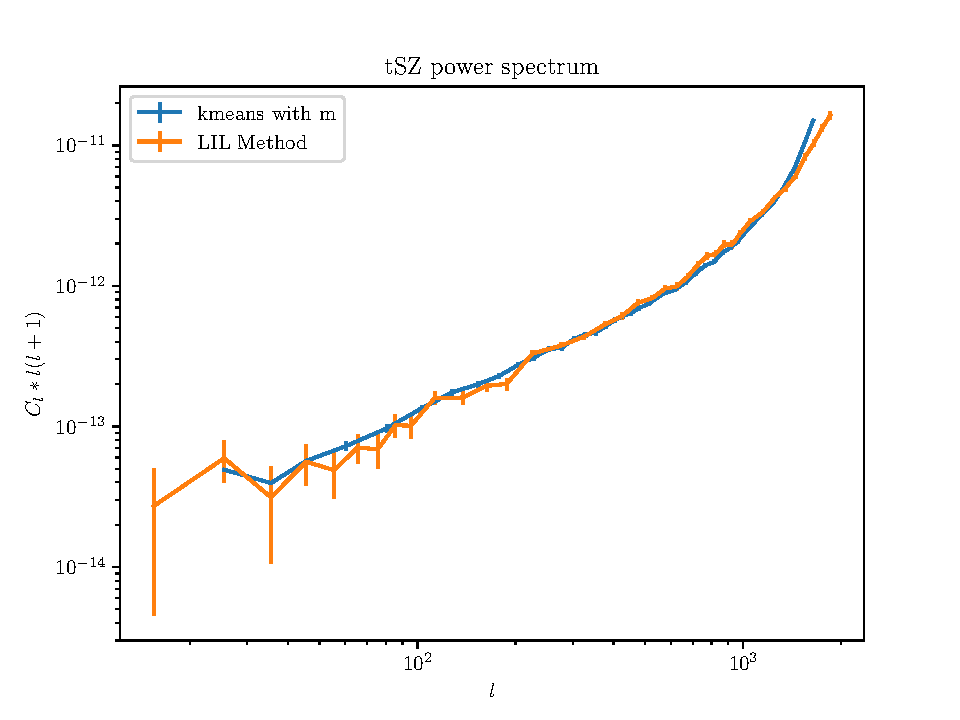
\includegraphics[width=0.7\linewidth]{sz_spec.pdf}
  \caption{Comparison of the tSZ power spectrum of Planck Data using various methods}
\end{figure}


%%% Local Variables:
%%% mode: latex
%%% TeX-master: "thesis"
%%% End:
